\begin{center}
    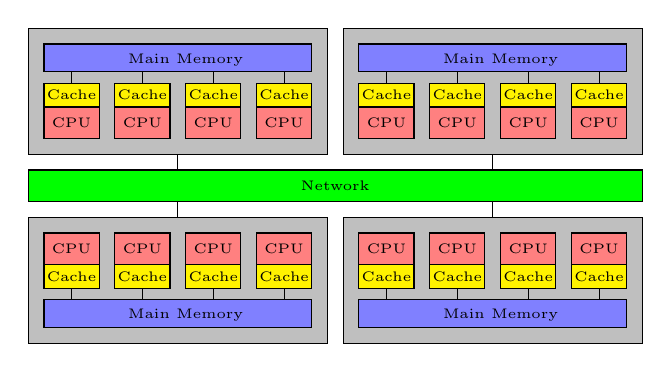
\begin{tikzpicture}[scale=0.2]
      \tikzstyle{every node}=[font=\tiny]
      \filldraw[fill=green] (0,9) rectangle (39,11);
      \draw (19.5,10) node {Network};
      % First Node
      \filldraw[fill=gray!50!white] (0,0) rectangle (19,8);
      \filldraw[fill=blue!50!white] (1,1) rectangle (18,2.75);
      \draw (10,1.75) node {Main Memory};
      % First Core
      \filldraw[fill=yellow] (1,3.5) rectangle (4.5,5.0);
      \draw (2.75,4.25) node {Cache};
      \filldraw[fill=red!50!white] (1,5.0) rectangle (4.5,7.0);
      \draw (2.75,6.0) node {CPU};
      \draw (2.75,3.5) -- (2.75,2.75);
      % Second Core
      \filldraw[fill=yellow] (5.5,3.5) rectangle (9.0,5.0);
      \draw (7.25,4.25) node {Cache};
      \filldraw[fill=red!50!white] (5.5,5.0) rectangle (9.0,7.0);
      \draw (7.25,6.0) node {CPU};
      \draw (7.25,3.5) -- (7.25,2.75);
      % Third Core
      \filldraw[fill=yellow] (10.0,3.5) rectangle (13.5,5.0);
      \draw (11.75,4.25) node {Cache};
      \filldraw[fill=red!50!white] (10.0,5.0) rectangle (13.5,7.0);
      \draw (11.75,6.0) node {CPU};
      \draw (11.75,3.5) -- (11.75,2.75);
      % Fourth Core
      \filldraw[fill=yellow] (14.5,3.5) rectangle (18.0,5.0);
      \draw (16.25,4.25) node {Cache};
      \filldraw[fill=red!50!white] (14.5,5.0) rectangle (18.0,7.0);
      \draw (16.25,6.0) node {CPU};
      \draw (16.25,3.5) -- (16.25,2.75);
      % Connect First Node to Network
      \draw (9.5,8) -- (9.5,9);

      % Second Node
      \filldraw[fill=gray!50!white] (20,0) rectangle (39,8);
      \filldraw[fill=blue!50!white] (21,1) rectangle (38,2.75);
      \draw (30,1.75) node {Main Memory};
      % First Core
      \filldraw[fill=yellow] (21,3.5) rectangle (24.5,5.0);
      \draw (22.75,4.25) node {Cache};
      \filldraw[fill=red!50!white] (21,5.0) rectangle (24.5,7.0);
      \draw (22.75,6.0) node {CPU};
      \draw (22.75,3.5) -- (22.75,2.75);
      % Second Core
      \filldraw[fill=yellow] (25.5,3.5) rectangle (29.0,5.0);
      \draw (27.25,4.25) node {Cache};
      \filldraw[fill=red!50!white] (25.5,5.0) rectangle (29.0,7.0);
      \draw (27.25,6.0) node {CPU};
      \draw (27.25,3.5) -- (27.25,2.75);
      % Third Core
      \filldraw[fill=yellow] (30.0,3.5) rectangle (33.5,5.0);
      \draw (31.75,4.25) node {Cache};
      \filldraw[fill=red!50!white] (30.0,5.0) rectangle (33.5,7.0);
      \draw (31.75,6.0) node {CPU};
      \draw (31.75,3.5) -- (31.75,2.75);
      % Fourth Core
      \filldraw[fill=yellow] (34.5,3.5) rectangle (38.0,5.0);
      \draw (36.25,4.25) node {Cache};
      \filldraw[fill=red!50!white] (34.5,5.0) rectangle (38.0,7.0);
      \draw (36.25,6.0) node {CPU};
      \draw (36.25,3.5) -- (36.25,2.75);
      % Connect Second Node to Network
      \draw (29.5,8) -- (29.5,9);

      % Third Node
      \filldraw[fill=gray!50!white] (0,12) rectangle (19,20);
      \filldraw[fill=blue!50!white] (1,17.25) rectangle (18,19);
      \draw (10,18.0) node {Main Memory};
      % First Core
      \filldraw[fill=yellow] (1,16.5) rectangle (4.5,15.0);
      \draw (2.75,15.75) node {Cache};
      \filldraw[fill=red!50!white] (1,15.0) rectangle (4.5,13.0);
      \draw (2.75,14.0) node {CPU};
      \draw (2.75,16.5) -- (2.75,17.25);
      % Second Core 
      \filldraw[fill=yellow] (5.5,16.5) rectangle (9.0,15.0);
      \draw (7.25,15.75) node {Cache};
      \filldraw[fill=red!50!white] (5.5,15.0) rectangle (9.0,13.0);
      \draw (7.25,14.0) node {CPU};
      \draw (7.25,16.5) -- (7.25,17.25);
      % Third Core 
      \filldraw[fill=yellow] (10.0,16.5) rectangle (13.5,15.0);
      \draw (11.75,15.75) node {Cache};
      \filldraw[fill=red!50!white] (10.0,15.0) rectangle (13.5,13.0);
      \draw (11.75,14.0) node {CPU};
      \draw (11.75,16.5) -- (11.75,17.25);
      % Fourth Core 
      \filldraw[fill=yellow] (14.5,16.5) rectangle (18.0,15.0);
      \draw (16.25,15.75) node {Cache};
      \filldraw[fill=red!50!white] (14.5,15.0) rectangle (18.0,13.0);
      \draw (16.25,14.0) node {CPU};
      \draw (16.25,16.5) -- (16.25,17.25);
      % Connect Third Node to Network
      \draw (9.5,11) -- (9.5,12);

      % Fourth Node
      \filldraw[fill=gray!50!white] (20,12) rectangle (39,20);
      \filldraw[fill=blue!50!white] (21,17.25) rectangle (38,19);
      \draw (30,18.0) node {Main Memory};
      % First Core
      \filldraw[fill=yellow] (21,16.5) rectangle (24.5,15.0);
      \draw (22.75,15.75) node {Cache};
      \filldraw[fill=red!50!white] (21,15.0) rectangle (24.5,13.0);
      \draw (22.75,14.0) node {CPU};
      \draw (22.75,16.5) -- (22.75,17.25);
      % Second Core 
      \filldraw[fill=yellow] (25.5,16.5) rectangle (29.0,15.0);
      \draw (27.25,15.75) node {Cache};
      \filldraw[fill=red!50!white] (25.5,15.0) rectangle (29.0,13.0);
      \draw (27.25,14.0) node {CPU};
      \draw (27.25,16.5) -- (27.25,17.25);
      % Third Core 
      \filldraw[fill=yellow] (30.0,16.5) rectangle (33.5,15.0);
      \draw (31.75,15.75) node {Cache};
      \filldraw[fill=red!50!white] (30.0,15.0) rectangle (33.5,13.0);
      \draw (31.75,14.0) node {CPU};
      \draw (31.75,16.5) -- (31.75,17.25);
      % Fourth Core 
      \filldraw[fill=yellow] (34.5,16.5) rectangle (38.0,15.0);
      \draw (36.25,15.75) node {Cache};
      \filldraw[fill=red!50!white] (34.5,15.0) rectangle (38.0,13.0);
      \draw (36.25,14.0) node {CPU};
      \draw (36.25,16.5) -- (36.25,17.25);
      % Connect Fourth Node to Network
      \draw (29.5,11) -- (29.5,12);
      
    \end{tikzpicture}
  \end{center}